\documentclass[phys,dissertation]{puthesis}

\usepackage{amsmath}
\usepackage{subfigure}
\usepackage{multicol}
\usepackage{multirow}
\usepackage{graphicx}
\usepackage{color}
\usepackage[square,comma,numbers]{natbib}
\usepackage[utf8]{inputenc}
\sloppy

\newcommand{\FIX}[1]{\textcolor{red}{$\left( \text{#1} \right)$}}

% Put % at the end of the last line to avoid getting an extra space
% in the abstract.
\title{
	Novel calibration methods for XENON1T
}

\author{Darryl Masson}{Masson, Darryl}

\pudegree{Doctor of Philosophy}{PhD}{April}{2016}

\majorprof{Rafael Lang}

\campus{West Lafayette}

% defs
\newcommand{\n}[1]{\mathrm{#1}}    % normal (roman) text in math mode
\newcommand{\1}[1]{\, \mathrm{#1}}
\newcommand{\dd}{\mathrm{d}}
\newcommand{\order}{\mathcal{O}}
\newcommand{\degree}{{}^{\circ}}
\newcommand{\arxiv}[1]{\href{http://arxiv.org/abs/#1}{\texttt{arXiv:#1}}}
\newcommand{\keVnr}{$\mathrm{keV_{nr}}$}
\newcommand{\keVee}{$\mathrm{keV_{ee}}$}
\newcommand{\ua}{$\mathrm{U_{A^{\prime}}}(1)$}

\newcommand{\err}[2]{$#1\,\pm\,#2$}

\newcommand{\Rn}{${}^{222}$Rn}
\newcommand{\Po}{${}^{218}$Po}
\newcommand{\Pb}{${}^{214}$Pb}
\newcommand{\BiPo}{${}^{214}$BiPo}
\newcommand{\todo}[1]{\color{red}\textbf{#1}\color{black}}

\begin{document}
\maketitle
\tableofcontents
\chapter{Prelim}
\section{Introduction}

It is now widely known that much of the universe is composed of matter that is not visible in telescopes observing across the entire range of electromagnetic radiation~\cite{Olive:2014,Blumenthal:1984,Clowe:2006eq}. Recent observations of the cosmic microwave background by WMAP~\cite{2013ApJS} and Planck~\cite{Ade:2015xua} have constrained the fraction of the universe that interacts with the CMB (and photons, in general) to ($4.86\pm0.16$)\%, but the fraction of the universe with mass (interacts with gravity) is ($30.89\pm0.62$)\%, indicating that about 85\% of the mass content of the universe is some new type of matter wholly unknown to modern science. One of the most favored candidates for this new matter is the Weakly Interacting Massive Particle (WIMP) model, which arises from a variety of extensions to the Standard Model~\cite{Jungman:1995df}. Other viable candidates include axions~\cite{2009PhRvD} or sterile neutrinos~\cite{Boyarsky:2009ix}, but as XENON1T is aimed primarily at the detection of WIMPs we will concern ourselves with that model.

Detectors based on liquid xenon (LXe) time-projection chambers (TPCs) are at the forefront of the search for dark matter. The best published limits on WIMP-nucleon interaction cross-sections for ``heavy'' WIMPs ($m_{\chi} > 10\1{GeV}/c^2$) were released recently by the LUX collaboration~\cite{Akerib:2015rjg}, based on $1.4\times10^4\1{kg}-\n{days}$ of exposure. Once it fully enters operation, the XENON1T detector will nominally reach this exposure within two weeks.

\section{TPC operation}

The operation of a dual-phase TPC is as follows: some interaction within the bulk of the liquid will free some electrons from a xenon atom. Some of these electrons will recombine instantly with the ion, resulting in scintillation light that will be observed by arrays of photomultiplier tubes (PMTs) installed on the top and bottom of the detector. This scintillation signal is generally referred to as the ``S1''. An electric field applied to the detector will cause some of the electrons to drift upwards towards the liquid-gas interface. Upon reaching this boundary, a stronger electric field accelerates the electrons quickly into the gas, causing energetic collisions with the atoms in the gas, resulting in a second signal observed by the PMTs. This second ionization signal is called the ``S2''. The time between the S1 and S2 indicates the length of time the electrons were drifting, which is a measurement of the depth of the event in the TPC. By analyzing the hit pattern on the top PMT array, the (x-y) location of the event can also be computed, yielding three-dimensional position reconstruction. The relative size of the S2 and S1 indicate a nuclear or electronic interaction. This process is shown schematically in figure~\ref{fig:tpcevent}.

\begin{figure}[htb]
\centering
\includegraphics[trim = 8cm 3cm 105mm 3cm, clip = true, width = 0.5\textwidth]{figures/idealized_event.pdf}
\caption{An idealized event in a dual-phase TPC.}
\label{fig:tpcevent}
\end{figure}

As the size of these detectors continues to grow to reach greater and greater sensitivities, new challenges arise in the accurate calibration of these devices. The XENON100 detector was calibrated by means of externally-placed sources~\cite{XENON100Collaboration2011}, and radiation from these penetrated sufficiently throughout the entire fiducial volume. While this method is still partially viable for nuclear recoil (NR) calibrations, it is no longer feasible for the case of electronic recoils (ER). Additionally, the increased size of XENON1T allows for some new opportunities of calibrations.

\section{NR calibrations}

While the XENON100 TPC is not significantly larger than the mean free path of fast neutrons (MeV~energies) in liquid xenon, XENON1T is 1~m in diameter, so it is now possible to resolve multiple scatters within the fiducial volume. This opens a new avenue for extremely accurate in-situ NR calibrations via the use of mono-energetic neutrons. Recall the elastic collision problem from kindergarten of a neutron onto a xenon atom initially at rest:
\begin{equation}
\frac{E_{Xe}}{E_n} = \frac{2\frac{m_{Xe}}{m_n}(1-\cos\theta)}{\left(1+\frac{m_{Xe}}{m_n}\right)^2}
\label{eq:collision}
\end{equation}

The ratio of energy deposited in the xenon atom to the energy of the incident neutron is a function of the ratio of masses and the rest-frame scattering angle, which can be calculated by measuring the locations of two interactions (assuming the source location is known). If the incident neutrons are mono-energetic, a very accurate measurement of the deposited energy can be found, and different calibration energies can be selected by changing the desired scattering angle.

To perform this calibration, a deuterium-deuterium fusion neutron generator was procured from NSD Fusion. When two deuterons collide with sufficient energy, they can fuse together via ${}^2\n{D} + {}^2\n{D} \rightarrow {}^3\n{He}\, (0.82\1{MeV}) + n \,(2.45\1{MeV})$, which has a 50\% branching ratio. The other reaction produces $^3$T and a proton. An alternate reaction is the DT reaction, ${}^2\n{D} + {}^3\n{T} \rightarrow {}^4\n{He} \,(3.6\1{MeV}) + n \,(14.1\1{MeV})$. The DD generator functions via inertial electrostatic confinement~\cite{Miley1997}, where deuterons are injected into a vacuum chamber and ionized. A cathode grid in the center of the chamber is held at some high voltage, causing the ions to fall into the center. Once a sufficient population of ions is achieved, a virtual anode is formed inside the cathode, which acts to further confine ions. Eventually, the ions in the center of the cage collide with sufficient energy to allow a reasonable probability of fusion.

The rate of fusion is a function of both the applied current and the applied cathode voltage. In order to study the response of the generator to these parameters, liquid scintillators containing EJ-301 were selected. This chemical is an organic liquid polymer with a high hydrogen density manufactured by Eljen Technologies, and is identical to the older and more well-known NE-213. EJ-301 is sensitive to both neutron and $\gamma$ radiation, so these two different signal responses must be separated in processing to discriminate between the desired neutron signals and the unwanted $\gamma$ background.

\subsection{Pulse Shape Discrimination}

While $\gamma$ interactions in EJ-301 excite atoms into a singlet state, neutron interactions result in triplet states~\cite{Kuchnir1968}. The triplet state decay transition is forbidden, so the state's lifetime is longer than that of the singlet. Based on this, a variety of processing algorithms can be implemented to discriminate between the two pulses based on their shapes. The oldest is the Charge Comparison Method, dating back to the prehistoric times of analog signal processing~\cite{Brooks1959}, and involves the use of two integration windows of different lengths, where the length of one window is generally tuned to match the shorter (singlet) decay mode, and the other to match the longer (triplet) decay mode. However, with the relatively recent rise of cheap digital storage and the availability of off-line processing, other methods have become possible, such as Fourier expansions, Laplace transforms, and fitting operations.

Each discrimination method assigns a value to each waveform, and the ``neutron-ness'' or ``$\gamma$-ness'' of the waveform is determined by that value. The quantification of the performance of a discrimination method has traditionally been done via the calculation of a Figure of Merit, based off the width and separation of the two (assumed) Gaussian populations of the discrimination parameter. However, this assumes the performance of the algorithms is largely independent of energy (except for some low-energy threshold). Thus, any algorithms offering better performance at higher energies will yield non-Gaussian populations and thus a larger population width, rendering merit-less the Figure of Merit. Additionally, the Figures of Merit are often reported without mention of the low-energy cut used. We propose a new method of quantifying the performance of these algorithms based off the energy-dependent acceptance of neutron events (or rejection of $\gamma$ events) at some confidence limit.

\section{ER calibrations}

The calibration of the electronic recoil response of XENON1T cannot be done in the same way as for XENON100. The mean free path of the 1.3~MeV $\gamma$-line from $^{60}$Co is only 70~mm, which is insufficient to penetrate throughout the fiducial volume of the TPC in a reasonable amount of time. Additionally, the 7~cm of xenon between the TPC and the inner cryostat very effectively shield the detector from external $\gamma$ radiation. Figure~\ref{fig:externalsource} shows the futility of this endeavor.

\begin{figure}[htb]
\centering
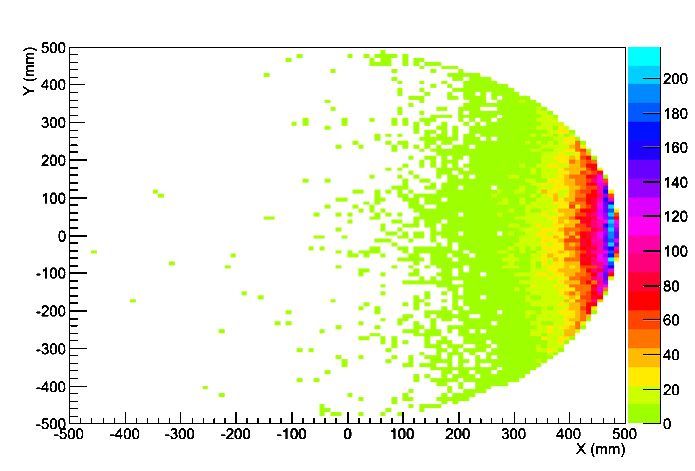
\includegraphics[trim = 0 0 0 0, clip = true, width = 0.6\textwidth]{figures/chapter_five/externalsource_dark_nostats.png}
\caption{Simulation of the distribution of events from an external $\gamma$ source. Given the fraction of events in the fiducial volume, it would take about a year to achieve sufficient statistics.}
\label{fig:externalsource}
\end{figure}

So, if the calibration cannot be performed from the outside, the only alternative is to perform it from the inside. However, one does not simply introduce radiation into the interior of a low-background detector filled with ultra-high purity xenon. Anything considered must:
\begin{itemize}
\item Get into the TPC
\item Do something useful
\item Go away
\end{itemize}

To get something into the TPC, it must either be able to hitchhike on some known contaminant of xenon (for instance, methane), or be a noble element. To make the activity go away, the isotope(s) must have relatively short half-lives, which would mean the activity decays away by itself, or the entire active volume must be recirculated through purification systems. However, as these detectors continue to grow in size, recirculation times will tend to increase, which means it is better if recirculation is not the preferred method of removing the activity from the detector.

For the isotope to do something useful while it is in the TPC, it needs to provide either some lines or some spectrum to calibrate the energy (in the first case) or the ER band (in the second). An isotope that provide one of these services $^{83m}$Kr (T$_{1/2}$ = 1.83~hr, Q-value 41.6~keV). Krypton is a noble element, and so can be introduced into the detector with ease. The two-step decay from the metastable excited state involves $\gamma$s of energy 32.2 and 9.4~keV with an intermediate half-life of 157~ns. These two lines can provide the energy calibration in the region of interest for a dark matter search, however they cannot perform the necessary ER band calibration. For this, low-energy $\gamma$-lines are unsuitable due to the very high stopping power of the liquid xenon. A Compton scatter from a higher-energy source would provide the desired spectrum, but so would a $\beta$ decay. A suitable isotope for this latter option is \Pb~(T$_{1/2}$ = 10.6~hr, Q-value 560~keV), which can be introduced into a detector via \Rn. This isotope is part of the decay chain of primordial $^{232}$Th, given in table~\ref{tab:th_chain}.

\begin{table}[htb]
\centering
	\begin{tabular}{| c | c | c | c | c |}
		\hline
		Isotope & Half-life & Decay mode & Q-value (keV) \\ \hline
		$^{232}$Th & $1.41\times10^{10}$ yr & $\alpha$ & 4081 \\ \hline
		$^{228}$Ra & 5.7 yr & $\beta$ & 46 \\ \hline
		$^{228}$Ac & 6.15 hr & $\beta$ & 2124 \\ \hline
		\Th & 1.9 yr & $\alpha$ & 5520 \\ \hline
		\Ra & 3.66 d & $\alpha$ & 5989 \\ \hline
		\Rn & 55.6 s & $\alpha$ & 6405 \\ \hline
		\Po & 0.145 s & $\alpha$ & 6906 \\ \hline
		\Pb & 10.6 h & $\beta$ & 570  \\ \hline
		\multirow{2}{*}{\Bi} & \multirow{2}{*}{61 m} & $\alpha$ (36\%)& 6207 \\
		& & $\beta$ (64\%)& 2252 \\ \hline
		\BiPo & 299 ns & $\alpha$ & 8954 \\ \hline
		\Tl & 3.1 m & $\beta$ & 4999 \\ \hline
		$^{208}$Pb & \multicolumn{3}{|c|}{Stable} \\
		\hline
	\end{tabular}
	\caption{The decay chain of primordial thorium, sometimes called the 4n series}
	\label{tab:th_chain}
\end{table}

One downside to the use of \Pb~is that only 12.3\% of decays go to the ground state of \Bi. The other decays are to excited states that decay with picosecond livetimes. As this is far below the temporal resolution limit of XENON1T, this will appear as a $\beta$ decay shifted to a higher energy. Additionally, the Q-value means that only a very small percentage of events ($\approx 1\%$ of decays) will have energy $<$20~keV necessary for calibration in the region of interest for a dark matter search. However, the half-life of \Pb~means that whatever activity we introduce into the TPC will decay away within a few days. This (and the general versatility of the decay chain) are more than enough to compensate for this. As \Rn~has a short half-life, sources of this isotope we acquired are based on \Th. However, \Th~does not decay directly into \Rn, but goes through \Ra~, and introducing this into the detector would lead to a much longer-lived background that must be avoided. Thus, limits must be placed on the release of these (and other) long-lived isotopes to prevent contamination of an otherwise low-background experiment. A variety of limits are published in~\cite{Lang:2016zde}, of which a subset are presented here for further discussion.

\subsection{Limits on the release of long-lived contaminants from the \Rn~source}

The \Rn~decay chain is versatile, producing $\alpha$-, $\beta$-, and $\gamma$-radiation that makes this source interesting for a wide range of applications. The source is ideal for calibration of intrinsic $^{222}$Rn backgrounds that are notoriously difficult to control in low-background experiments. High-energy alphas~\cite{WeberM:2013,Albert:2015vma} and $^{212}$Bi/$^{212}$Po decays~\cite{Bellini:2012qg} can be used to accurately understand intrinsic backgrounds. The relatively short half-life of $^{216}$Po (145~ms) allows for the measurement of currents or liquid flows within the bulk of the detector volume. Using position reconstruction algorithms that yield the positions of the decays of \Rn~and $^{216}$Po together with the time difference between these two decays, allows for a measurement of the drift velocity of polonium ions~\cite{Albert:2015vma}. Thus, currents within the bulk of the detector can be mapped to identify possible dead regions that do not participate in the recirculation of the active volume through purification systems. Additionally, the high-energy $\alpha$ lines can be used to probe regions in a detector with poor light or charge collection efficiency. Further, the $^{208}$Tl decay produces a $2.6\1{MeV}$ $\gamma$-line, very close to the Q-value of $^{136}$Xe double-beta decay. This line will be accompanied by the $\beta$ energy and usually by simultaneous $\gamma$-lines (mostly $580\1{keV}$), which results in steps in the calibration spectrum (e.g. at $\approx 3.2\1{MeV}$) above the $^{136}$Xe Q-value. Finally, $\beta$-decays of the chain that go to the ground state can be used to calibrate the low-energy response of dark matter detectors. While the high Q-value of the $^{212}$Bi $\beta$-decay (2.2~MeV) and short half-life of the daughter $^{212}$Po (300~ns) render that decay unsuitable for this purpose, the $\beta$-decay of \Pb~(12.3\% branching ratio to ground state, Q-value 560~keV) is very suitable for this task, as shown in Figure~\ref{fig:pb212spectrum}.

\begin{figure}[htb]
\centering
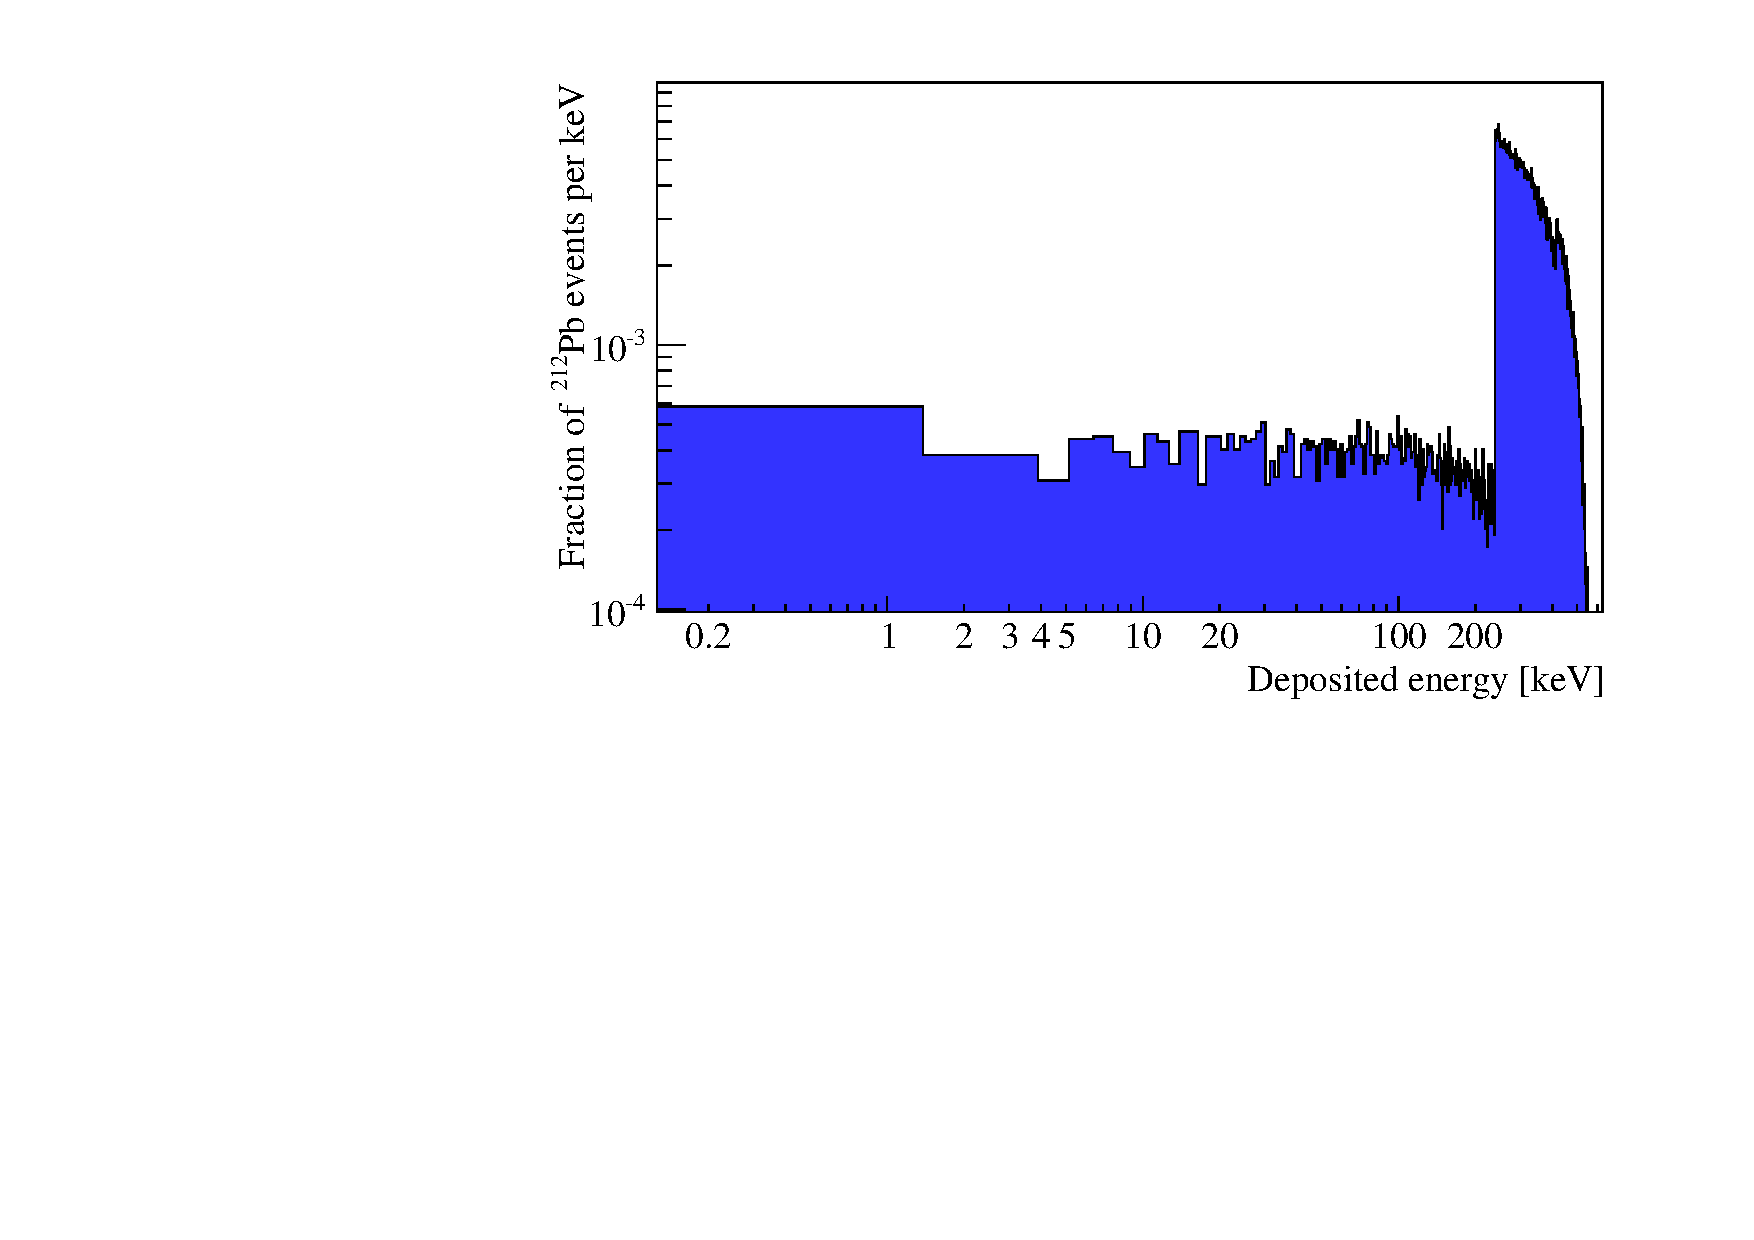
\includegraphics[trim = 5 0 50 15, clip = true,width = 0.8\columnwidth]{figures/chapter_five/pb212_spectrum.pdf}
\caption{A simulation of the $\beta$-spectrum of \Pb. The feature at 240 keV is due to decay modes with an associated $\gamma$ that adds to the energy observed in the decay.}
\label{fig:pb212spectrum}
\end{figure}

A major advantage of our source is that the time scale of the \Rn~decay chain is dominated by the relatively short half-life of \Pb~($T_{1/2}=10.66\1{hours}$). Thus, the introduced activity can completely decay away within a few days, making this source useful even for the largest anticipated liquid detectors~\cite{Baudis:2012,Akerib:2015cja,Franco:2015pha}. As both \Th~($T_{1/2}=1.9\1{years}$) and \Ra~($T_{1/2}=3.6\1{days}$) have much longer half-lives, emanation of these isotopes from the source must be limited. Also, isotopic contamination with $^{230}$Th in the $^{228}$Th source itself can lead to the emanation of $^{222}$Rn ($T_{1/2}=3.8\1{days}$) which has to be avoided.

Here, we use a variety of methods to derive limits on the release of long-lived isotopes, and demonstrate that these sources are suitable for the calibration of even next-generation low-background experiments. Open \Rn~sources were produced by electroplating thorium nitrate, $\n{Th}(\n{NO}_3)_4$, onto the center of a $30\1{mm}$ diameter stainless steel disk in a bath of 1M nitric acid ($\n{HNO}_3$). A ring of width 2.5~mm around the edge of the disk was left for mounting purposes. The activity was $40\1{kBq}$ as of March, 2015. Each source is held in a small stainless steel vessel to attach it to a noble gas recirculation system using 1/2"~VCR piping, see figure~\ref{fig:th228source}.

\begin{figure}[htb]
\centering
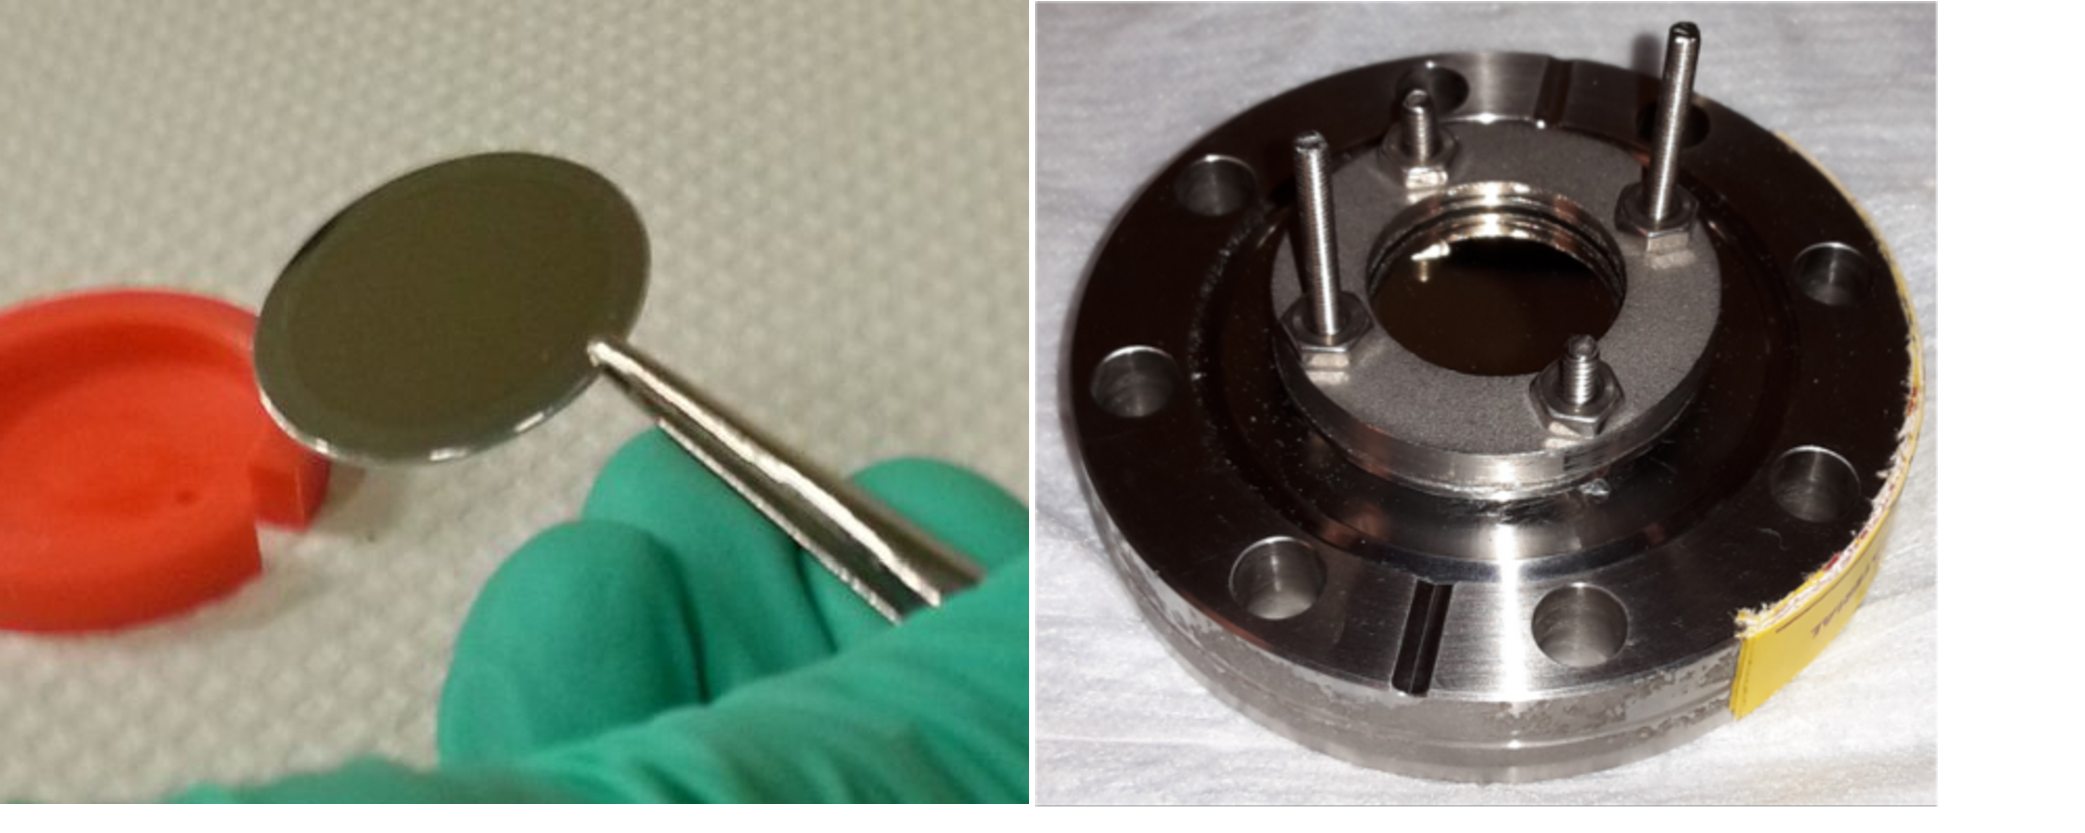
\includegraphics[trim = 5 10 50 0, clip = true,width = 0.8\columnwidth]{figures/chapter_five/source_image.pdf}
\caption{\Th~is deposited onto a $30\1{mm}$ stainless steel disc (left). It is held in a simple emanation vessel (right) for mounting on a noble gas system.}
\label{fig:th228source}
\end{figure}

\subsubsection{$\gamma$-Measurements of Filter Deposition}
\label{sec:tuv}

% TUV measurement
The source was tested for the release of \Ra~and \Th~using a standard procedure. Nitrogen was flushed through the source vessel for 96 hours. A filter of type ML050/0 was mounted inline $18\1{cm}$ after the source, containing a filter paper on which any released radionuclides could be deposited. This filter paper was then tested for $\gamma$-activity with a high-purity germanium detector. A first measurement was made immediately after exposure, and a second measurement a week later, see Table~\ref{tab:tuv}.

\begin{table}[htb]
\centering
\caption{Measurements of radionuclide release from the \Rn~source collected in filter paper.}
\label{tab:tuv}
\renewcommand{\arraystretch}{1.2}
\begin{tabular}[c]{|llcc|}
\hline\hline
\multicolumn{2}{|l}{Measurement} & 1 & 2 \\
\multicolumn{2}{|l}{Time after exposure} & Immediate & 1 week \\
\multicolumn{2}{|l}{Livetime} & $375\1{s}$ & $11500\1{s}$ \\ \hline
\multirow{5}{*}{Activity/Bq}
& \Th & $<35$ & $<1.97$ \\
& \Ra & $<6$ & $<0.61$ \\
& \Pb & $87\pm11$ & $<0.07$ \\
& $^{212}$Bi & $84\pm34$ & $<0.68$ \\
& $^{208}$Tl & $28\pm5$ & $<0.07$ \\
\hline\hline
\end{tabular}
\end{table}

Both the exposure time and the time between measurements are significant compared to the half-life of \Ra. We account for both the decay during these intervals as well as the production of \Ra~from the decay of \Th. The week between the two measurements is more than 15 half-lives of \Pb, hence any recorded activity of its daughters $^{212}$Bi or $^{208}$Tl in the second measurement would have been from the decay of \Ra, not any initial population of \Pb. We use the lowest measurement (here, \Pb) to constrain the release of \Ra~from the source to $<0.43\1{atoms/s}$ and that of \Th~to or $<22\1{atoms/s}$. Scaling these values for the activity of the source yields a stray emanation of $<0.66\1{atoms/min/kBq}$ \Ra~and $<34\1{atoms/min/kBq}$ \Th. We choose these units (atoms/min/kBq) to account for the decay of the sources over the time the various measurements were made, and to allow comparisons between the sources.

The obvious limitation of this measurement is that there may have been radium or thorium released by the source but not caught by the filter, in which case the given limits must be scaled by the efficiency of the filter. Additionally, any thorium or radium plated out on the pipes connecting the source vessel and the filter would not show up in this measurement.

% Jochen's measurements
A similar but more sensitive experiment was performed by pumping nitrogen at 1 standard liter per minute (slpm) for 9 days in a closed loop through the \Rn~source vessel. The source was followed by a MILLEX-FG 50 filter at a distance of 8~cm, containing a $0.2\1{\mu m}$ PTFE filter membrane. The exposure time brought any released \Ra~nearly into equilibrium on the filter and gave potential \Th~more time to deposit itself. After exposure, the filter membrane was tested for $\gamma$-activity with high-purity germanium detectors~\cite{Budjas:1,Budjas:2}. A spectrum of these measurements is shown in figure~\ref{fig:gammaspectrum}. A simulation of the germanium crystal detector geometry performed in GEANT4~\cite{Geant4} indicated an efficiency of 6.5\% at 240 keV.

\begin{figure}[htb]
\centering
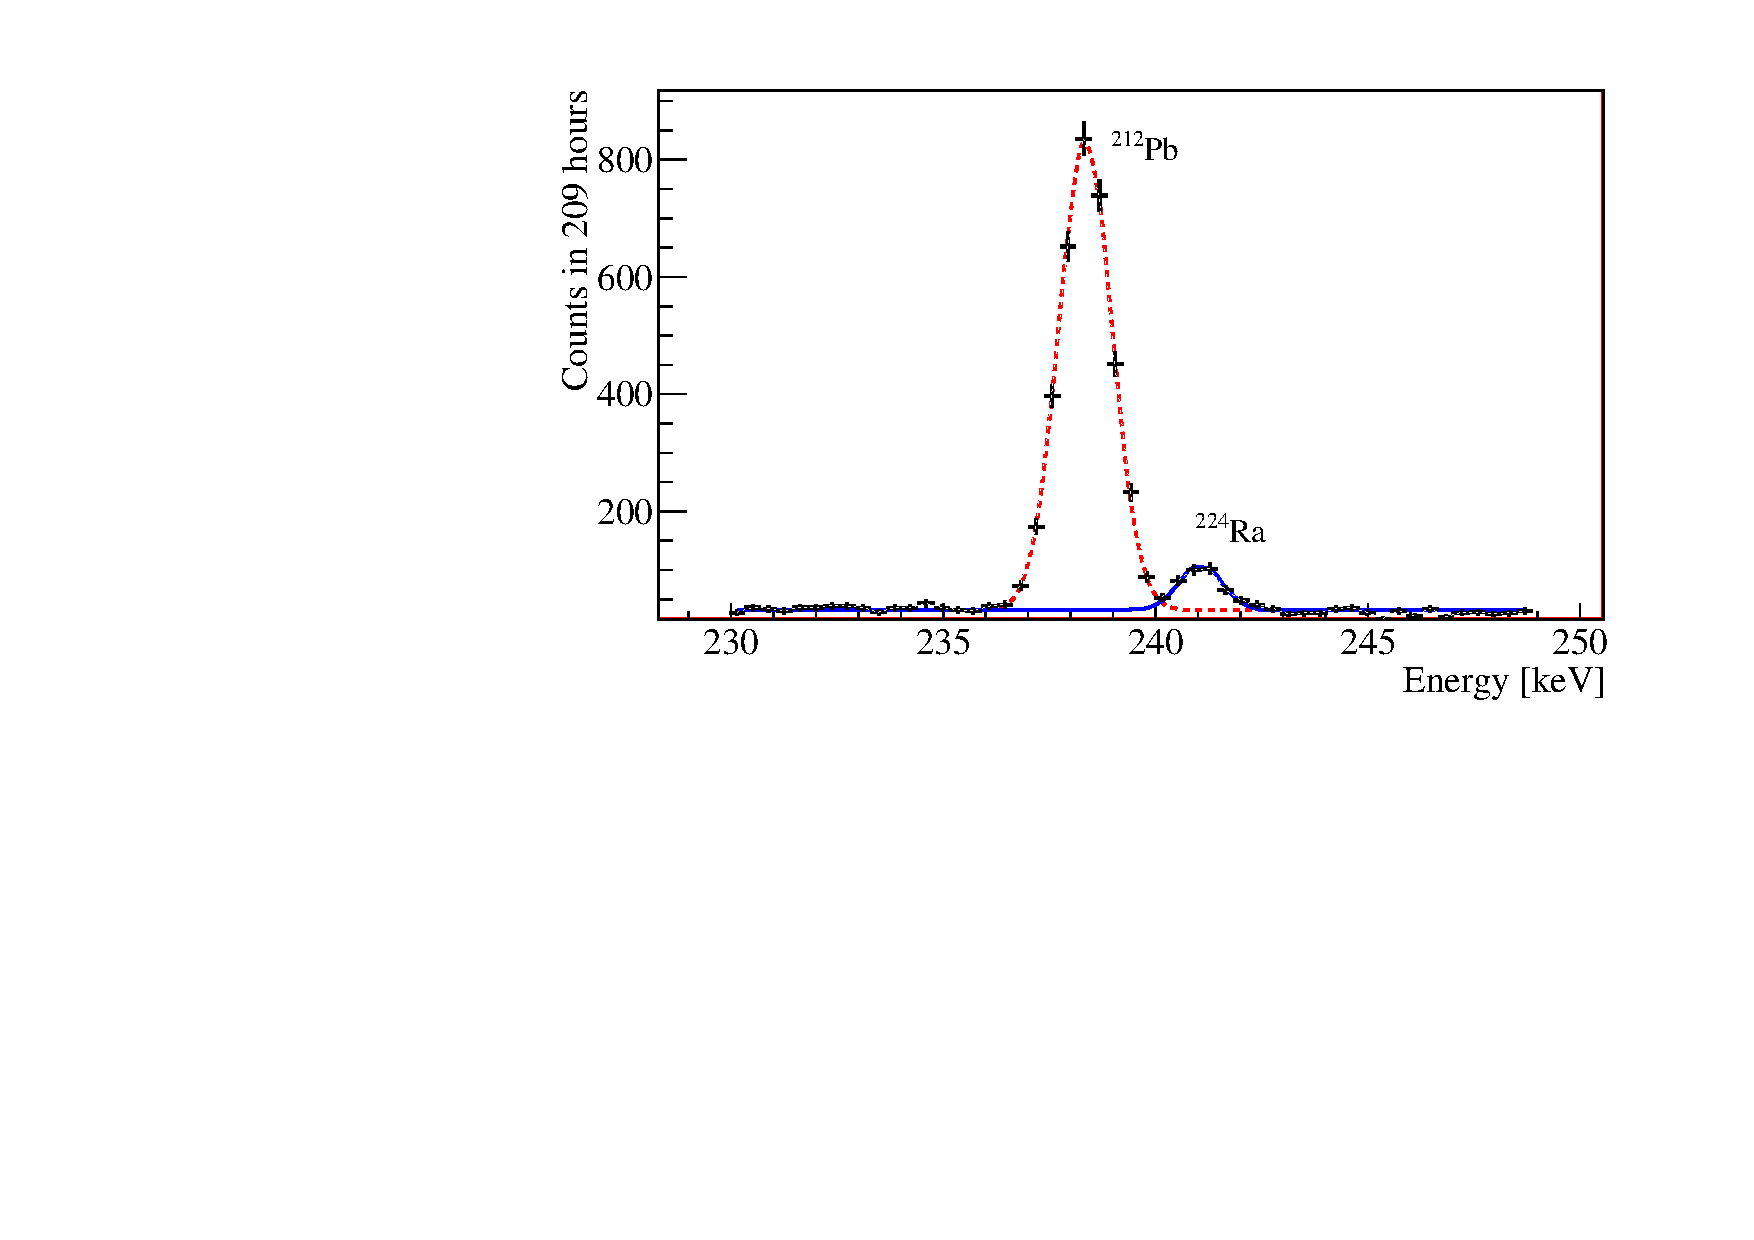
\includegraphics[trim = 15 0 50 20, clip = true,width = 0.8\columnwidth]{figures/chapter_five/ge_spectrum.pdf}
\caption{Gamma spectrum taken of the filter 7.2 days after exposure showing the \Pb~line at 238.6 keV and the \Ra~line at 241.0 keV. The dashed and solid lines are from a fit to the data.}
\label{fig:gammaspectrum}
\end{figure}

A week after exposure most of the \Pb~has decayed and measurements become sensitive to \Ra. A measurement with a livetime of 208 hours yielded a \Ra~activity of $(1.0\pm0.3)\1{Bq}$ on the filter at the end of exposure. A second measurement was done forty-two days after exposure, at which point the \Ra~deposited on the filter should have decayed to $3\times10^{-4}$ of the initial population. Thus, any measured \Ra~activity could be attributed to residual \Th. We calculate upper limits (90\% CL) of 2.5 mBq for \Th~and 2.4 mBq for \Ra~on the filter. These activities convert to emanation rates of $(1.9\pm0.6)\1{atoms/min/kBq}$ \Ra~and $<0.4\1{atoms/min/kBq}$ \Th.

% Argon flushing measurement
\subsubsection{$\gamma$-Spectroscopy of Pipe Contamination}
\label{sec:flush}

A test of radium plate-out was performed by flushing argon from a high-pressure tank through a pressure regulator, the source vessel, and then a copper pipe of $6\1{mm}$ diameter and $50\1{cm}$ length. The argon flow averaged $6\1{slpm}$ though with sizable fluctuations. After 41~hours of flushing, the copper pipe was cold-welded shut at both ends to seal in any materials deposited on the inner surface, and swiftly transported for measurement using our low-background germanium counters. Several measurements were done over the course of about two months to determine the $\gamma$-activity of the copper pipe. The results of the measurements are given in Table~\ref{tab:flush_meas}.

\begin{table}[htb]
\centering
\caption{Results of the measured $\gamma$-activity in the cold-welded copper pipe after flushing argon through source and pipe.}
\label{tab:flush_meas}
\renewcommand{\arraystretch}{1.2}
\begin{tabular}{|llccc|}
\hline\hline
\multicolumn{2}{|l}{Measurement} & 1 & 2 & 3 \\
\multicolumn{2}{|l}{Time after exposure} & 10 hours & 7 days & 68 days \\
\multicolumn{2}{|l}{Livetime} & 76733 s & 897820 s & 357802 s \\ \hline
\multirow{2}{*}{Activity [Bq]}
& \Ra & N/A & $0.25\pm0.03$ & $<0.088$ \\
& \Pb & $13.8\pm0.1$ & $0.215\pm0.005$ & $<0.088$ \\
\hline\hline
\end{tabular}
\end{table}

The interpretation of these data is done in a very similar way to that presented in the previous section. The first measurement started approximately 1 half-life of \Pb~after exposure, so any amount deposited on the pipe would still be observable. By the time the second measurement was started, a week had passed ($>$15 half-lives), so any initial \Pb~would have decayed to a negligible amount, making the measurement sensitive to potential \Pb~from the decay of \Ra. The interval between exposure and the third measurement is many half-lives of \Ra, making the measurement sensitive to potential contamination from the parent \Th~in the copper pipe. The calculated results are give in table~\ref{tab:flush_limits}.

\begin{table}[htb]
\centering
\caption{Calculated values and limits on \Ra~and \Th~release from deposition in the copper pipe after argon flushing.}
\label{tab:flush_limits}
\renewcommand{\arraystretch}{1.2}
\begin{tabular}{|lcc|}
\hline\hline
Isotope & Activity after exposure & Emanation rate \\ \hline
\Pb & $(26.0\pm0.2)\1{Bq}$ & N/A \\
\Ra & $(0.95\pm0.11)\1{Bq}$ & $(1.53\pm0.04)\1{atoms/min/kBq}$ \\
\Th & $<0.093\1{Bq}$ & $<47\1{atoms/min/kBq}$ \\
\hline\hline
\end{tabular}
\end{table}

Indeed trace amounts of \Ra~appear to have come off the source in this experiment. While the overall activity is very small, it motivates the use of an additional filter just after the source vessel for the calibration of low background detectors.

% Alpha spec at Purdue
\subsubsection{Measurements of Filter Efficacy}
\label{sec:filter}

In order to assess the performance of various filters in limiting the release of \Ra~from the \Rn~source, the source vessel was connected to a xenon gas system. Xenon gas was recirculated through various configurations involving the \Rn~source vessel, filters, and a Si PIN diode as an $\alpha$-spectrometer~\cite{Bray}. The source was exposed to the xenon gas stream for a few days, then bypassed, and the decaying activity monitored to measure any released radium. Two filter types were tested for their ability to remove radium from the gas stream. The first filter was a Swagelok F-series 0.5-micron sintered filter, the second was a Swagelok SCF-series ceramic filter.

The source vessel was connected directly to the sintered filter and then to the Si PIN diode with about $1\1{m}$ of 1/4" stainless steel pipe. For the ceramic filter, the extra piping was reduced to 8 cm. Xenon gas at $1\1{barg}$ was recirculated through the gas system at $5\1{slpm}$ for the sintered filter and $10\1{slpm}$ for the ceramic filter. After exposure with the sintered filter in line, the source and filter were bypassed and recirculation continued through the detector vessel for several weeks. After exposure with the ceramic filter, recirculation was stopped and the activity deposited in the detector vessel left to decay. Figure~\ref{fig:bipo} shows the activity of coincident $^{212}$Bi-$^{212}$Po (BiPo) activity in the Si PIN diode for the measurement of the ceramic filter from when the source was opened to three days after the source was closed, when the detector vessel was evacuated.

\begin{figure}[htb]
\centering
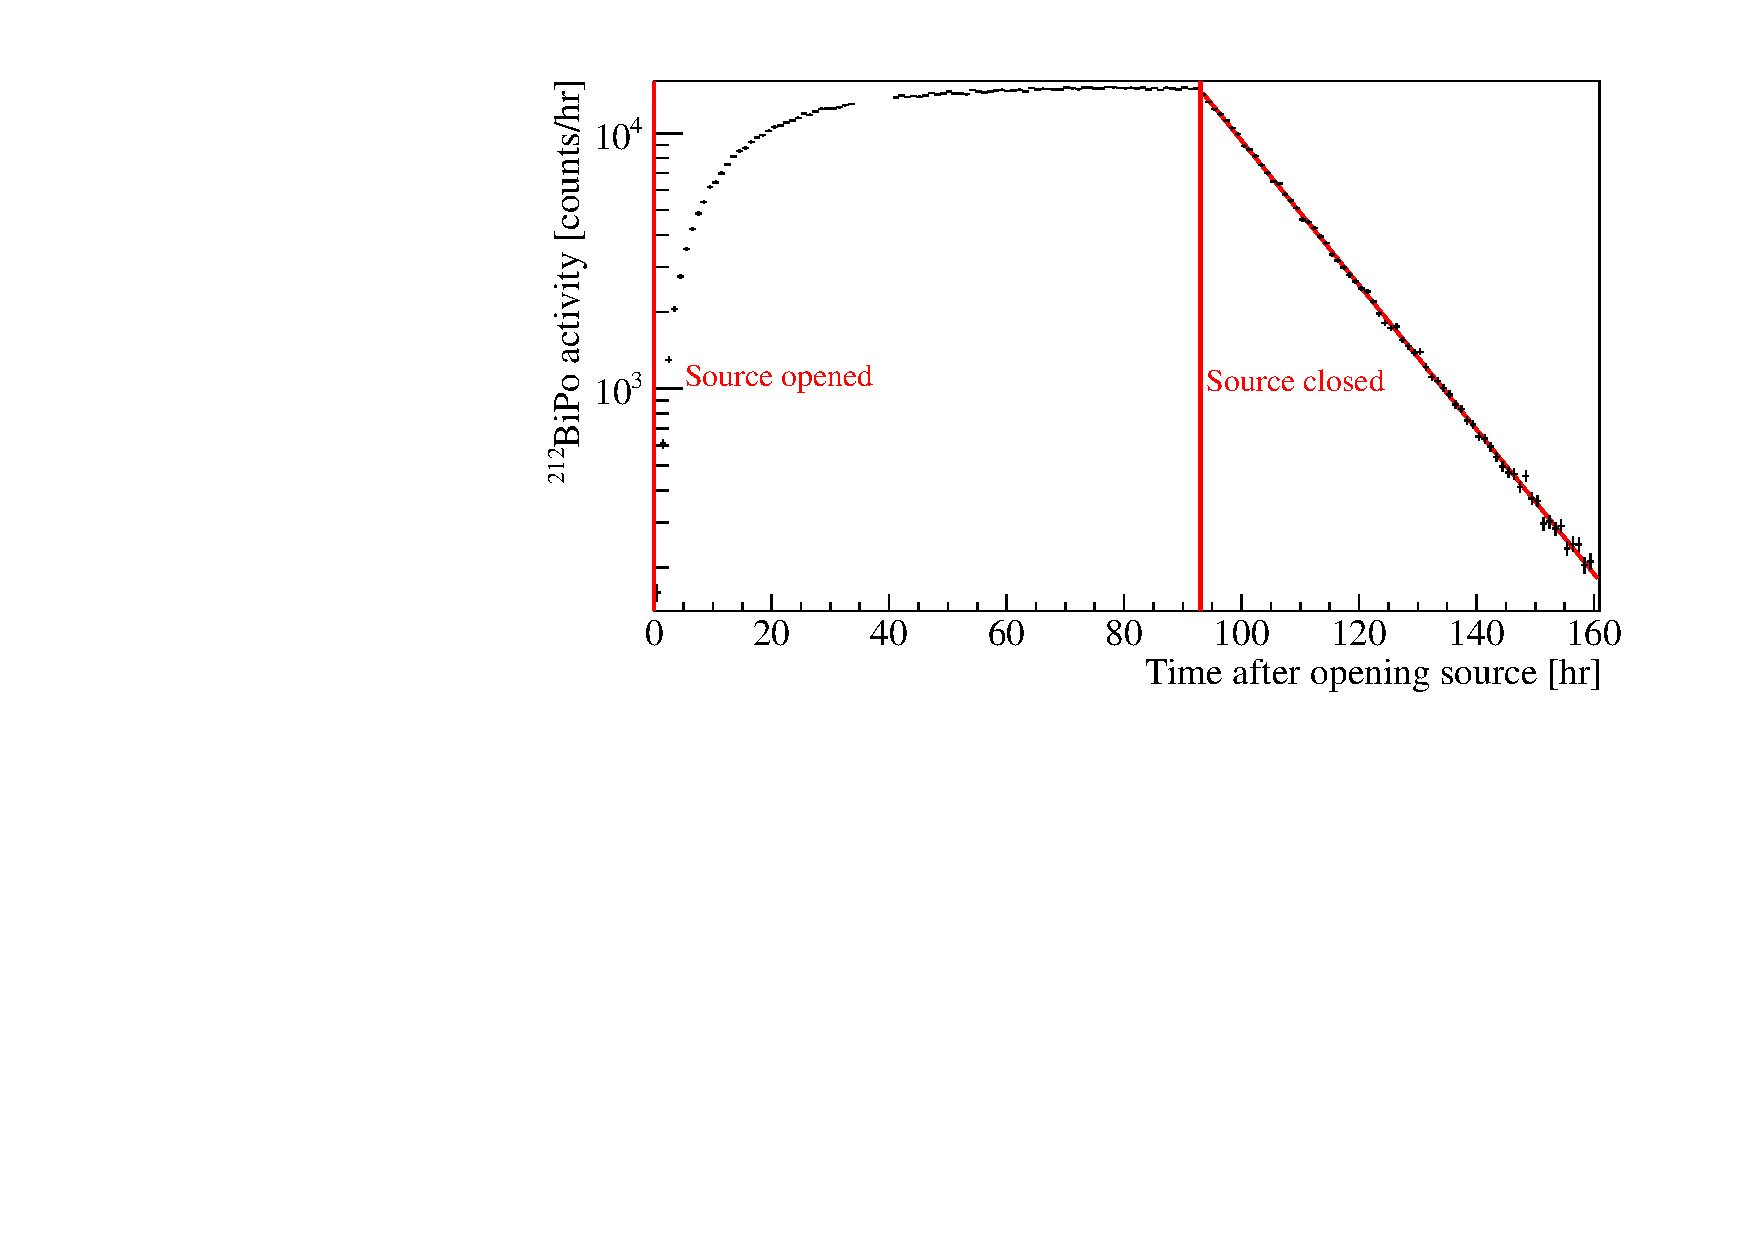
\includegraphics[trim = 5 5 40 15, clip = true,width = 0.8\columnwidth]{figures/chapter_five/bipo_activity.pdf}
\caption{Activity of $^{212}$BiPo in the Si PIN diode during and after flushing xenon through the ceramic filter. An exponential was fitted to the decaying part, yielding a half-life of $(10.64\pm0.05)\1{h}$ in excellent agreement with the \Pb~half-life of $(10.64\pm0.01)\1{h}$~\cite{Firestone}.}
\label{fig:bipo}
\end{figure}

The activity in the Si PIN diode was monitored as the released \Pb~decayed to background levels. A summary of the results are given in Table~\ref{tab:filter_limits}. About 14 half-lives after closing the source the \Pb~has almost completely decayed to background levels, at which point any measurement would be sensitive to the release of \Ra. The background rate of $^{212}$BiPo events was found prior to these measurements to be $(42\pm7)\1{\mu Bq}$. Figure~\ref{fig:bipo_background} shows the decay for the measurement of the sintered filter, along with a fitted exponential and constant.

\begin{figure}[htb]
\centering
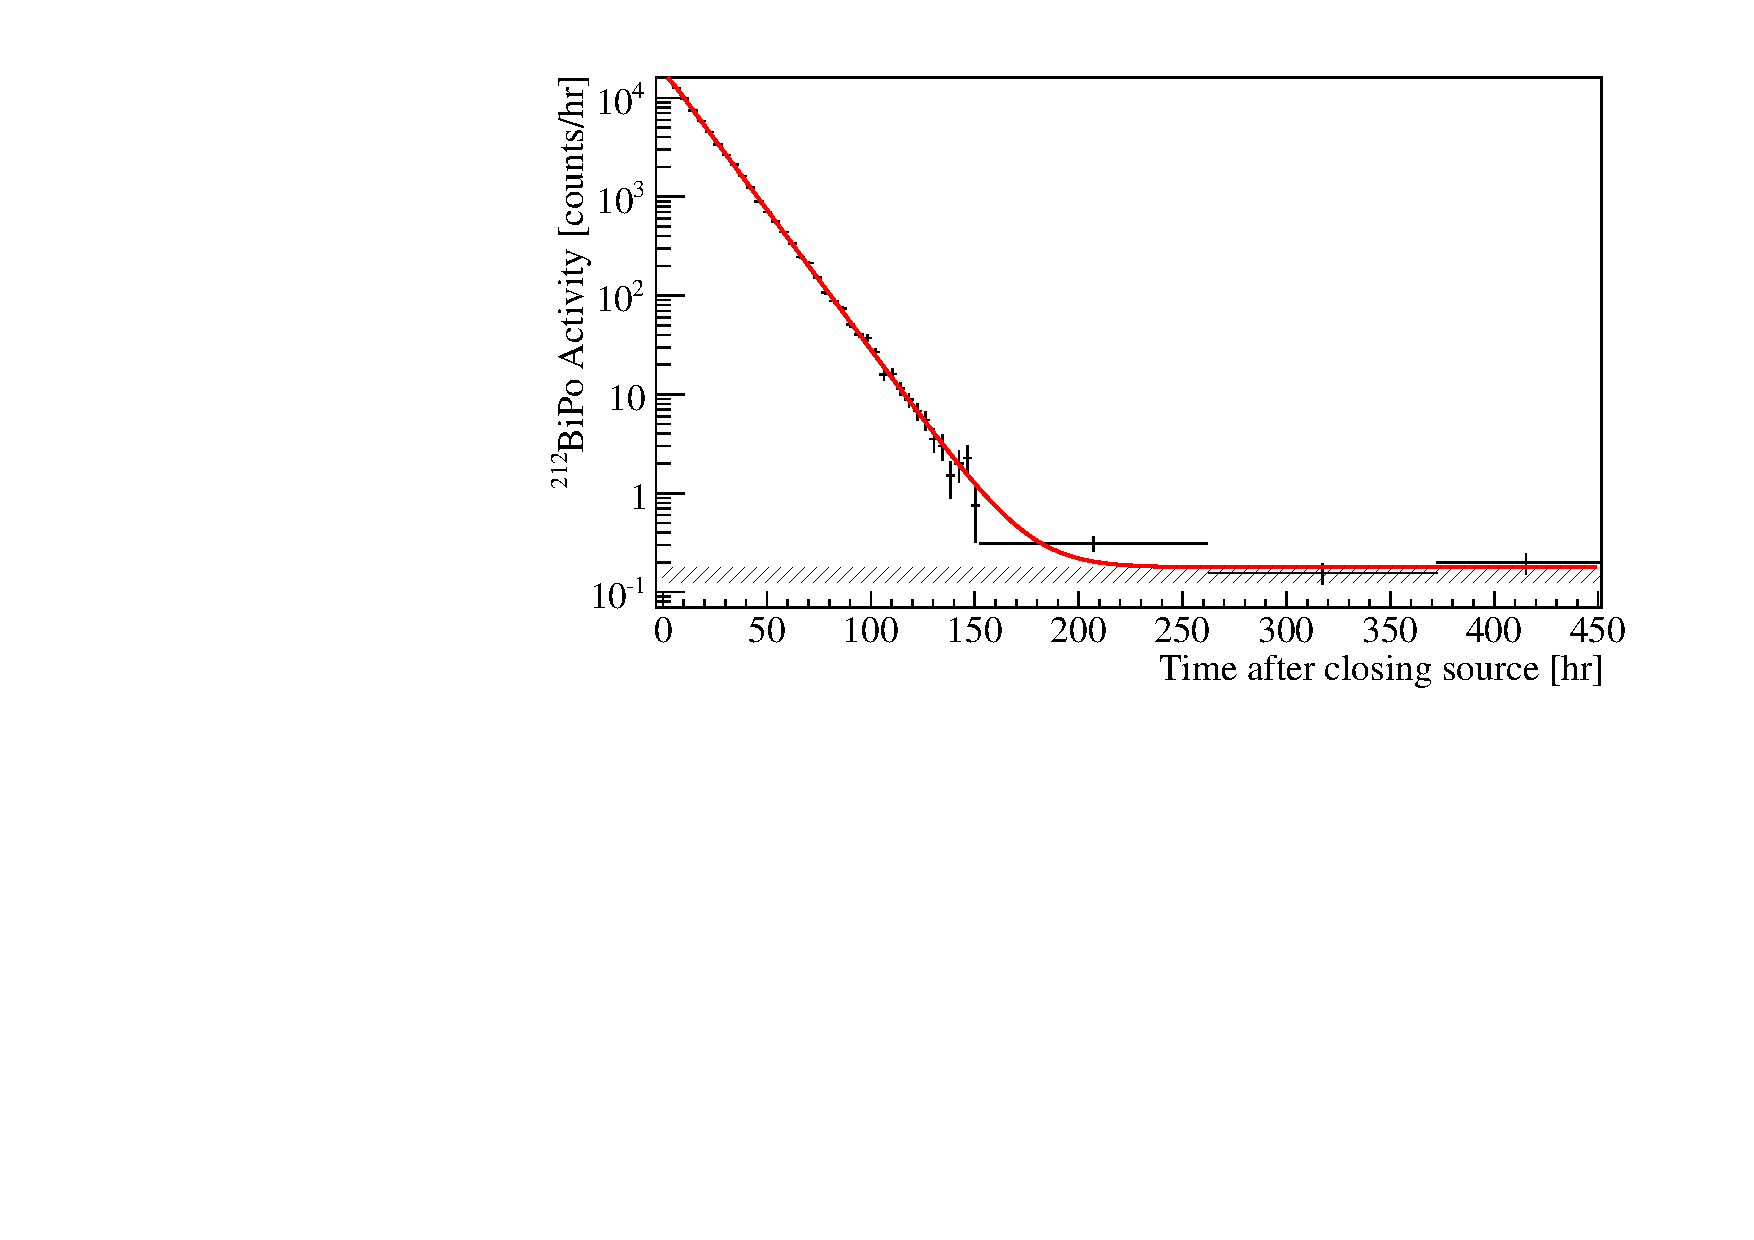
\includegraphics[trim = 10 5 40 15, clip = true,width = 0.8\columnwidth]{figures/chapter_five/bipo_background_sintered.pdf}
\caption{Decay to background of $^{212}$BiPo in the Si PIN diode for the measurement of the sintered filter. An exponential and a constant are fitted to the data. The band is the previously measured background of the detector.}
\label{fig:bipo_background}
\end{figure}

\begin{table}[htb]
\centering
\caption{Measurement results for the 0.5 micron sintered and ceramic filters}
\label{tab:filter_limits}
\renewcommand{\arraystretch}{1.2}
\begin{tabular}{|lccc|}
\hline\hline
Filter & Exposure & Fitted half-life & Fitted background \\ \hline
Sintered & $39\1{hr}$ & $(10.64\pm0.11)\1{hr}$ & $(49\pm8)\1{\mu Bq}$\\
Ceramic & $93\1{hr}$ & $(10.51\pm0.60)\1{hr}$ & $(46\pm8)\1{\mu Bq}$\\
\hline\hline
\end{tabular}
\end{table}

Both background values show some increase over the rate measured before this experiment, but in neither case is the increase statistically significant ($1\sigma$ for the sintered filter, $0.43\sigma$ for the ceramic filter). However, we can still (conservatively) attribute these small increases to some released \Ra, in which case we can limit the release of \Ra~to $<0.65\1{atoms/day/kBq}$ for the sintered filter and $<0.21\1{atoms/day/kBq}$ for the ceramic filter. Thus we see that both filters are highly effective at preventing the release of $^{224}$Ra from the source.

A more direct measurement of filter efficiency was performed by placing two identical 90~micron sintered filters in series in the gas system immediately after the source vessel. After recirculating xenon gas at 6.5~slpm through the source and filters for 100~hours, the two filters were then placed on top of the Si PIN diode to measure any $\alpha$-activity coming off of them that could be attributed to \Ra. A total of 4~days of data were taken. The spectra of the two filters is shown in Figure~\ref{fig:twofilters}. While the first filter showed an activity of $(55.4\pm2.1)\1{mBq}$ of \Ra, the second filter that was placed immediately downstream of the first only showed an activity of $(1.63\pm0.18)\1{mBq}$ of \Ra. Both numbers are corrected for the activity at the time of source closing. Hence, their ratio directly gives the filter efficiency. This value is independent of systematic uncertainties such as the collection efficiency of the Si PIN diode, geometrical effects, etc. We thus find these 90~micron sintered filters to retain $(97.1\pm0.3)$\% of \Ra~flushing through them.

\begin{figure}[htb]
\centering
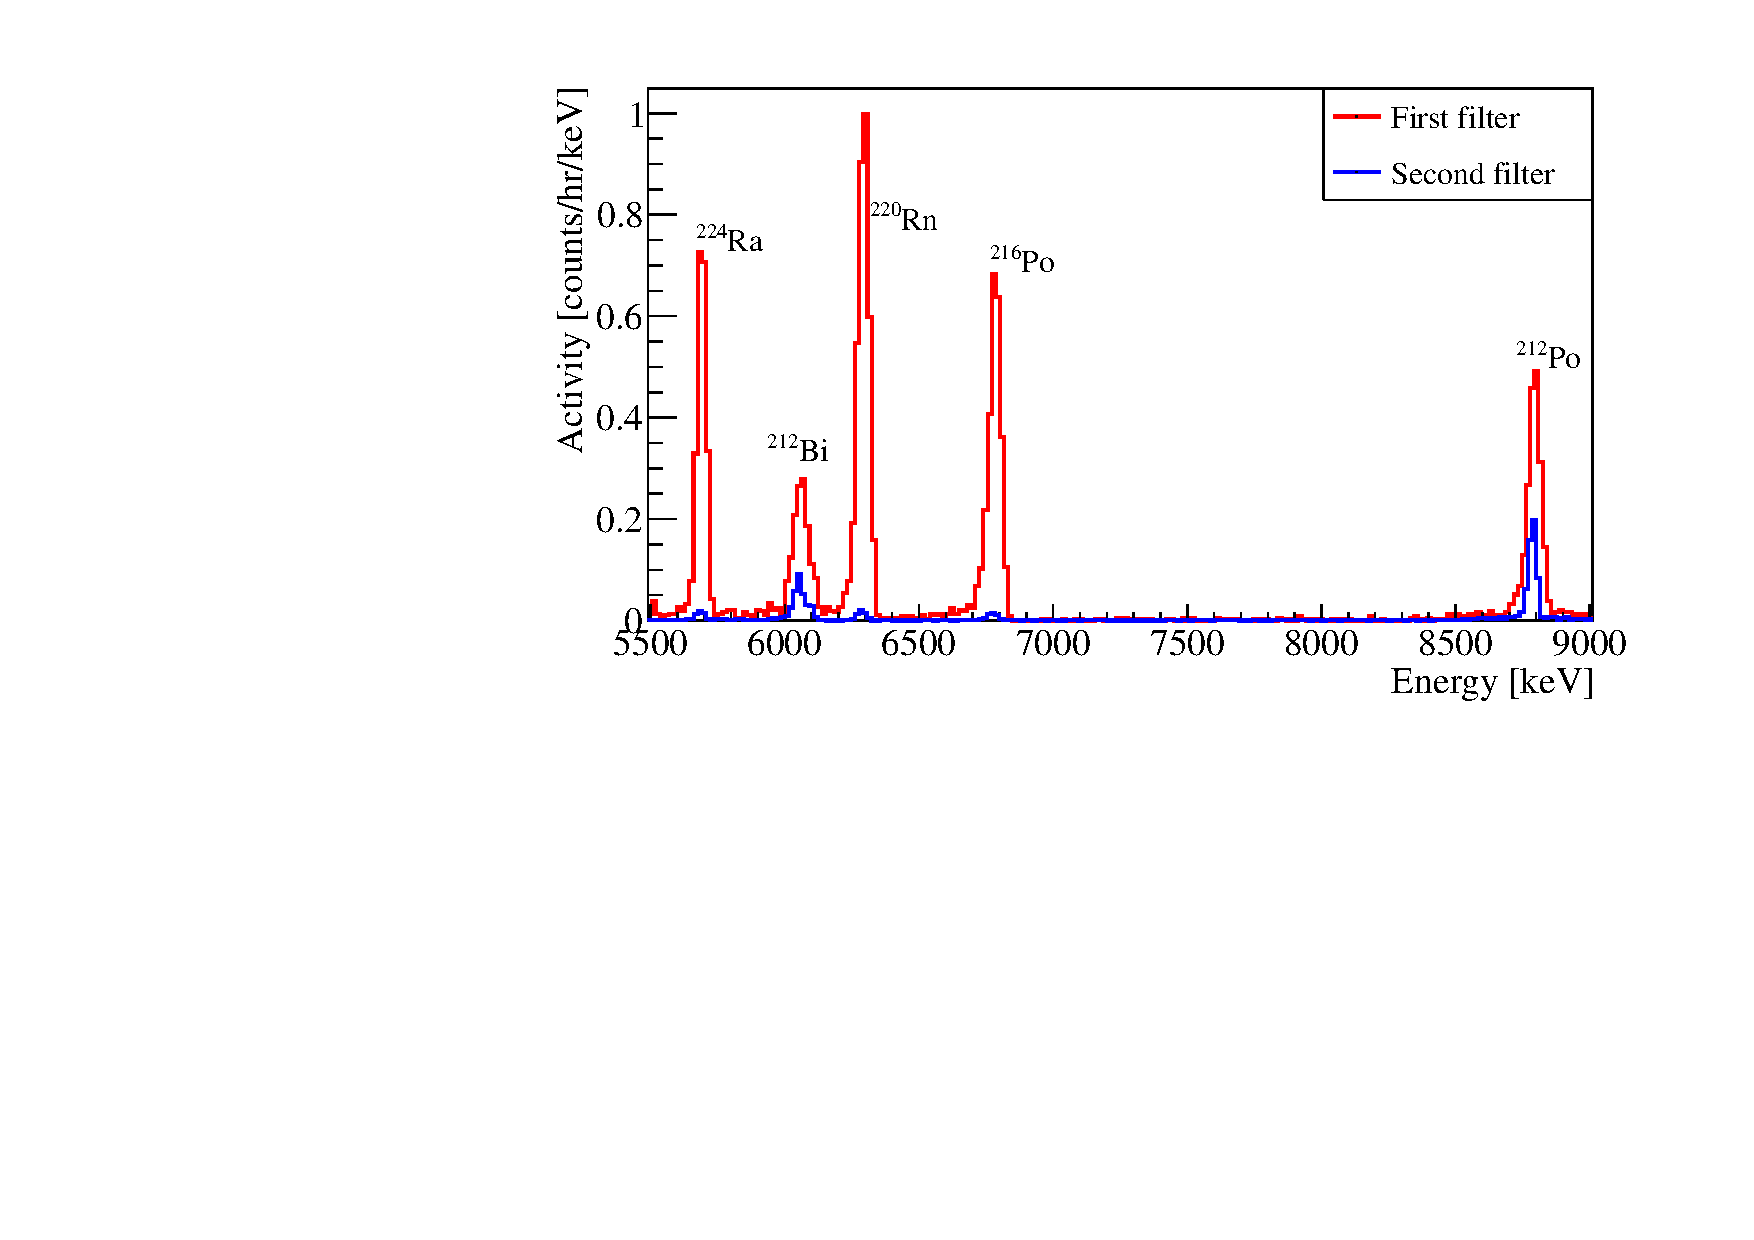
\includegraphics[trim = 5 0 40 20, clip = true,width = 0.8\columnwidth]{figures/chapter_five/twofilters.pdf}
\caption{Energy spectrum taken with the Si PIN diode from two sintered filters that were placed in series directly after the source in a xenon gas recirculation system.}
\label{fig:twofilters}
\end{figure}

\subsubsection{Interpretation}

\begin{table}[htb]
\centering
	\caption{Summary of all measurements of emanation rates, given in units of atoms/min/kBq.}
	\label{tab:summary}
	\begin{tabular}{|lcc|}
		\hline \hline
		Measurement & \Th & \Ra \\ \hline
		$\gamma$ measurements of filters  & $<34$ & $<0.66$ \\
		& $<0.4$ & $1.9\pm0.6$ \\
		Pipe contamination & $<47$ & $1.53\pm0.04$ \\
		Sintered filter & N/A & $<4.5\times10^{-4}$ \\
		Ceramic filter & N/A & $<1.5\times10^{-4}$ \\
		\hline \hline
	\end{tabular}
\end{table}

Table~\ref{tab:summary} summarizes the various measurements. The two $\gamma$ measurements of filter deposition and the measurement of pipe contamination are methodologically very similar, yet the results are strikingly different. The apparent inconsistency between the $\gamma$ measurements and pipe contamination can be attributed to deposition of \Ra~in the 1/2" piping: in the first two measurements, 18~cm and 8~cm of piping were present respectively in between the source vessel and filter, while the copper pipe was less than 1~cm from the source (leaving just enough space to cold-weld the copper). In the second $\gamma$ measurement, the flow through the source vessel and the filter was laminar, whereas the flow was turbulent for the pipe contamination measurement. Due to its extremely high reactivity, radium will bond readily to pipe walls. This is facilitated by turbulent flow, while in laminar flow the slow process of radial diffusion will impede the plate-out of \Ra. As the second $\gamma$ measurement and the pipe contamination measurement are consistent, we attribute the discrepancy of the first $\gamma$ measurement to the different conditions of the gas flow.

For the measurements of filter efficiency, the limits presented for the ceramic and 0.5~micron sintered filters are very satisfactory, while in the two-filter measurement, the 90~micron sintered filters are only 97\% efficient. However, at the time of this measurement, the source had an activity of around 60~kBq. Hence, the activity seen in the first filter ($55.4\pm2.1\1{mBq}$) shows a drastic reduction in the activity after only a few centimeters of piping. From this, we can conclude that only a vanishing percentage of these contaminants make it out of the source vessel. With these sources being used in a fluid stream, one may thus expect the vast majority of \Ra~and \Th~to plate out in any connecting piping.

\section{Future work}

While the preliminary work in characterizing these various new sources (neutron generator and \Rn~source) has largely been completed, they have yet to be deployed on XENON1T. There is a wealth of information to be gained by the analysis of data collected with these two sources, and we expect Purdue to take a leading role in this once XENON1T is operational and collecting data.

Additionally, a question yet unanswered pertains to the planned XENONnT upgrade and its successor, DARWIN. A 2.4~MeV neutron has a mean free path in liquid xenon of about 17~cm, which means we can expect a reasonable number of double-scatters within the fiducial volume from an externally-placed neutron source. However, this will only barely be effective for the XENONnT TPC, which is anticipated to have a diameter approximately 25~cm greater than XENON1T. For the planned 40-tonne DARWIN detector, this is no longer feasible. The question remains as to how the nuclear recoil calibration will be performed on DARWIN, and some new methods need to be proposed and tested to address this. Some ideas include using higher-energy neutrons (such as the 14 MeV neutrons produced from deuterium-tritium reactions) which have a longer mean free path, or embedding a neutron emitter in some nanomaterial to absorb the nuclear recoil and dissolving these into the active volume. Proofs of concept of these ideas need to be tested to determine suitable methods for calibration of detectors in the 10-tonne scale.

\bibliographystyle{aps}
\bibliography{library}

\end{document}